\chapter{Analysis}\label{anal_ch}

\section{Self tracking}
%\textbf{COMMENT: Elaborate this to motivate the project and explain the background.}
Experience Sampling Method (ESM) and Ecological Momentary Assessment (EMA) are the research methodologies that refer to the usage of self tracking\cite{esm}. What defines these methods are the use of collecting real world data in the moment, whether that be psychological (thoughts, feelings, mood, pain etc) or physical (food/drinks consumed, sneezing, cramps etc). Traditionally this had been achieved with diaries, which could have the same set of questions printed on each page designed to collect the desired data. In modern times digital diaries have been created, for example as apps on smartphones and smartwatches. The benefit of these methods is that the prevent recall bias, since the data is collected in the moment (or shortly after) compared to daily diaries where a user by the end of the day has to think back and recall the data. The more time passed between the event and the time the data is collected, the larger the risk of recall bias will be, and the data can even be forgotten.

When collecting data that requires active self tracking, there will always be a burden involved. The simpler the data is to collect, the smaller the burden can be. For example tracking each time a person sneezes only requires a time stamp which can be collected by wearing a smartbutton like the one made by Larsen et al.\cite{eg}. On the other hand, if tracking the pain levels of a patient, the patient needs a way to input that on scale preferably a VAS. One solution has been to create a digital VAS on a smartphone or smartwatch, similar to the work of Kami\'nski\cite{tomas}. Compared to the smartbutton, this solution has a much higher burden, the user must turn the display on, navigate the software to input the value and it requires a user's full attention to execute. With the improvements Dam-Jensen\cite{dam} introduced, the burden was lowered to only have the user press, hold and release a button while doing an arm gesture.

As a evolution to the design of Dam-Jensen\cite{dam}, this thesis will introduce a self tracking method where the user will follow the same gestures (described later in this Chapter) and press a button only once (not press, hold and release). This new method will reduce the burden even further compared to the other mentioned methods.










\section{Usage of VAS}
In Figure \ref{real_vas} we see one of the VAS rulers that is sold to and used by hospitals to measure the pain levels of patients, while they come in different designs their principals are the same. On one side of the ruler we see 5-6 faces with expression going from happy to discomfort to sad and crying, these expression are meant to illustrate the amount of pain and are often displayed together with a text description explaining the feeling of pain as seen in Figure \ref{vas_faces}. On the other side of the VAS ruler there is regular ruler of 10cm (sometimes shown as 100mm instead). On the ruler there is a slider, the patient will be shown the side of the ruler with the faces, and asked to adjust the slider to fit the level of pain they experience, on the backside the slider will indicate a position on the ruler from 0 (no pain) to 10 (most pain), this position is then registered by a doctor or nurse as the pain level. The VAS is not limited to measuring pain, it can be used for any subjective characteristics or attitudes that cannot be directly measured, for example mood, annoyance, anxiety, but the measuring of pain is the most common use of VAS.

\begin{figure}[h!]
    \centering
    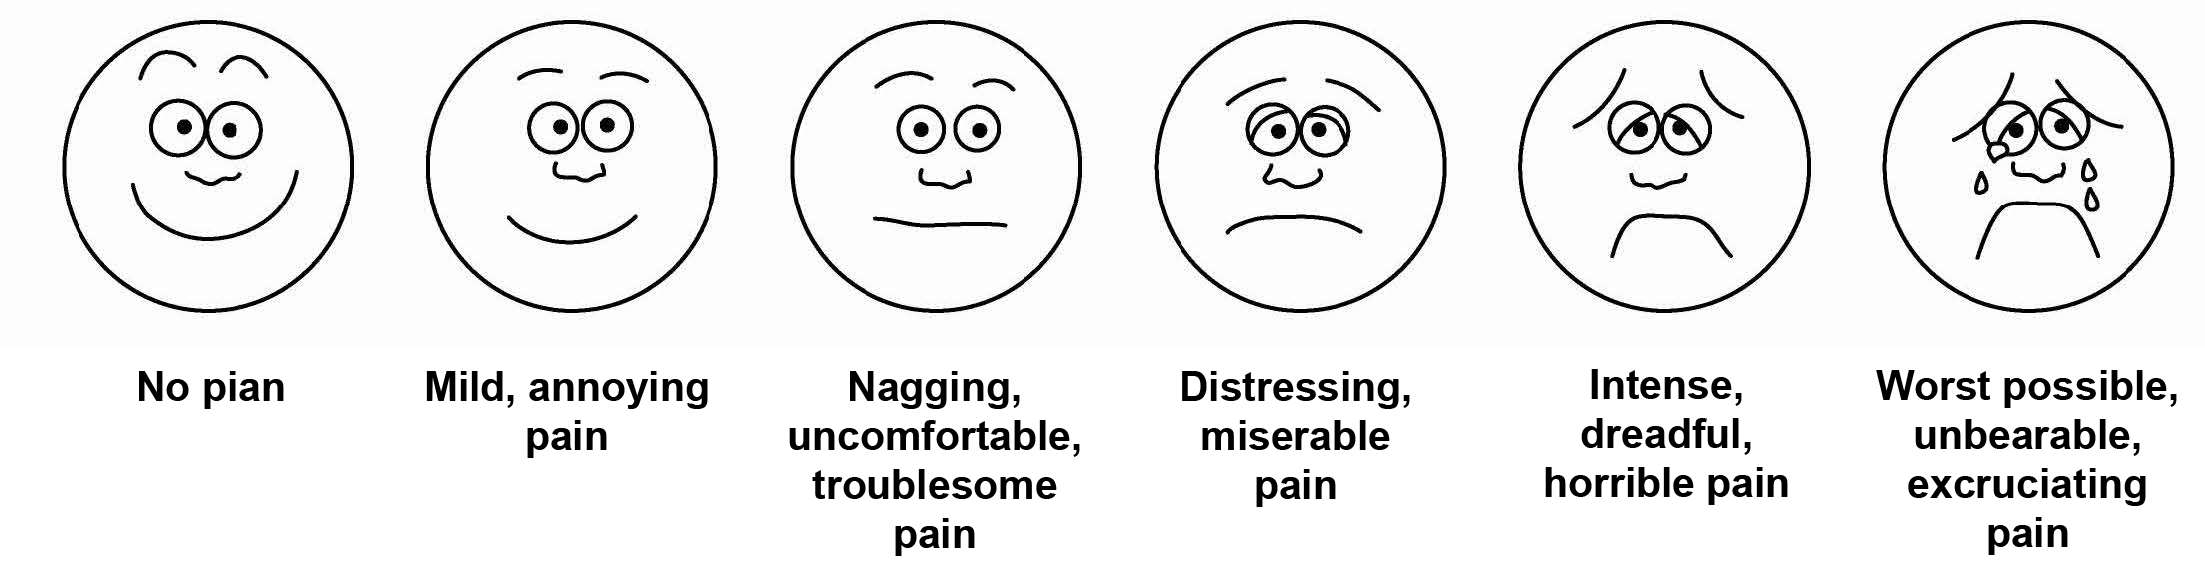
\includegraphics[width=0.75\textwidth]{figures/vas_faces.png}
    \caption{Example of faces and descriptions on VAS for measuring pain\cite{vas_faces}}
    \label{vas_faces}
\end{figure}

The VAS can be compared to the Likert scale\cite{likert} and Borg scale\cite{borg_scale}, but what makes the VAS different is that it is continuous where the others are discrete. Evidence show that VAS have better metrical characteristics compared to discrete scales and therefor a wider range of statistical methods can be applied to the measurements\cite{best_scale}.

Despite its benefits VAS are a burden to use, even digital version since the require a screen and attention. It is therefor interesting to investigate if other solutions with less burden can perform equally or better than the VAS.








\section{Orientation in 3D space}
Before creating a device that translates the orientation of the hand to a scale, one must first understand orientation in 3D space. We can rotate an object around each of its 3 axis, these actions are refereed to as pitch, roll and yaw. In Figure \ref{plane} we see an illustrations of these rotations performed on a airplane.

Pitch is rotation around the axis across the airplane, this rotation can be felt during takeoff and climbing (shortly after the wheels lift of the ground) of a airplane, where the pitch is dramatically changed from 0º (parallel to the ground) to $\thicksim$15-20º\cite{takeoff}.

Roll is rotation around the axis along the airplane, this rotation can sometimes be felt when an airplane has to perform a sharp turn and then rolls a little to one side so one wing tip is higher in the air than the other (when airplanes turn the yaw will also change), this rotational movement where the airplane rolls over is the roll axis.

Yaw is the rotation around the last axis, the same axis you would measure the height of airplane on. This rotation is barely felt in a airplane, but it is this orientation that will change the direction of the airplane, from lets say facing north to facing west by rotating 90º to the left (from the pilots perspective).

Getting the orientation of an object is then a matter of measuring the pitch, roll and yaw, there a different ways to do this and they will be discusses a little later, for now we will measure each rotation in degrees and define the orientation of 0º pitch, 0º roll and 0º yaw to be an object that is level in both directions and facing north. A full rotation in one axis is 360º and would leave the object in the same position as it started out. This definition is very similar to Euler angles witch will be discussed further.

\begin{figure}[h!]
    \centering
    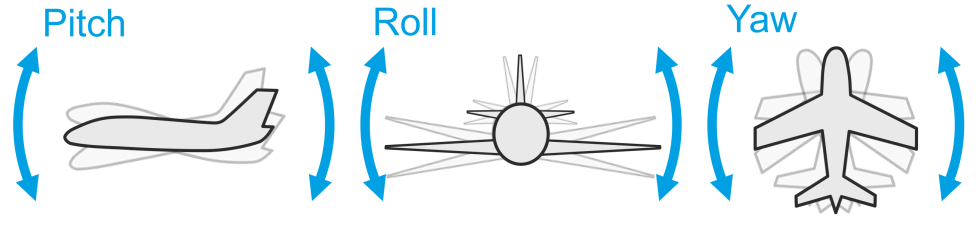
\includegraphics[width=1\textwidth]{figures/pitch_rool_yaw_v2.png}
    \caption{Pitch, roll and yaw of an airplane (edited version of figure found online\cite{plane})}
    \label{plane}
\end{figure}

\subsection{Orientation of the arm}
With the orientation defined as the rotation of the three axis, we need to translate this into movement of the arm. In Figure \ref{pitch}, \ref{roll} and \ref{yaw} the movement to adjust pitch, roll and yaw is described.

Pitch is changed by rotating the arm around the elbow, resulting in the lower arm being raised/lowered. The angle between the lower arm and table (horizontal plane) is then the measurement for this rotation.

\begin{figure}[h!]
    \centering
    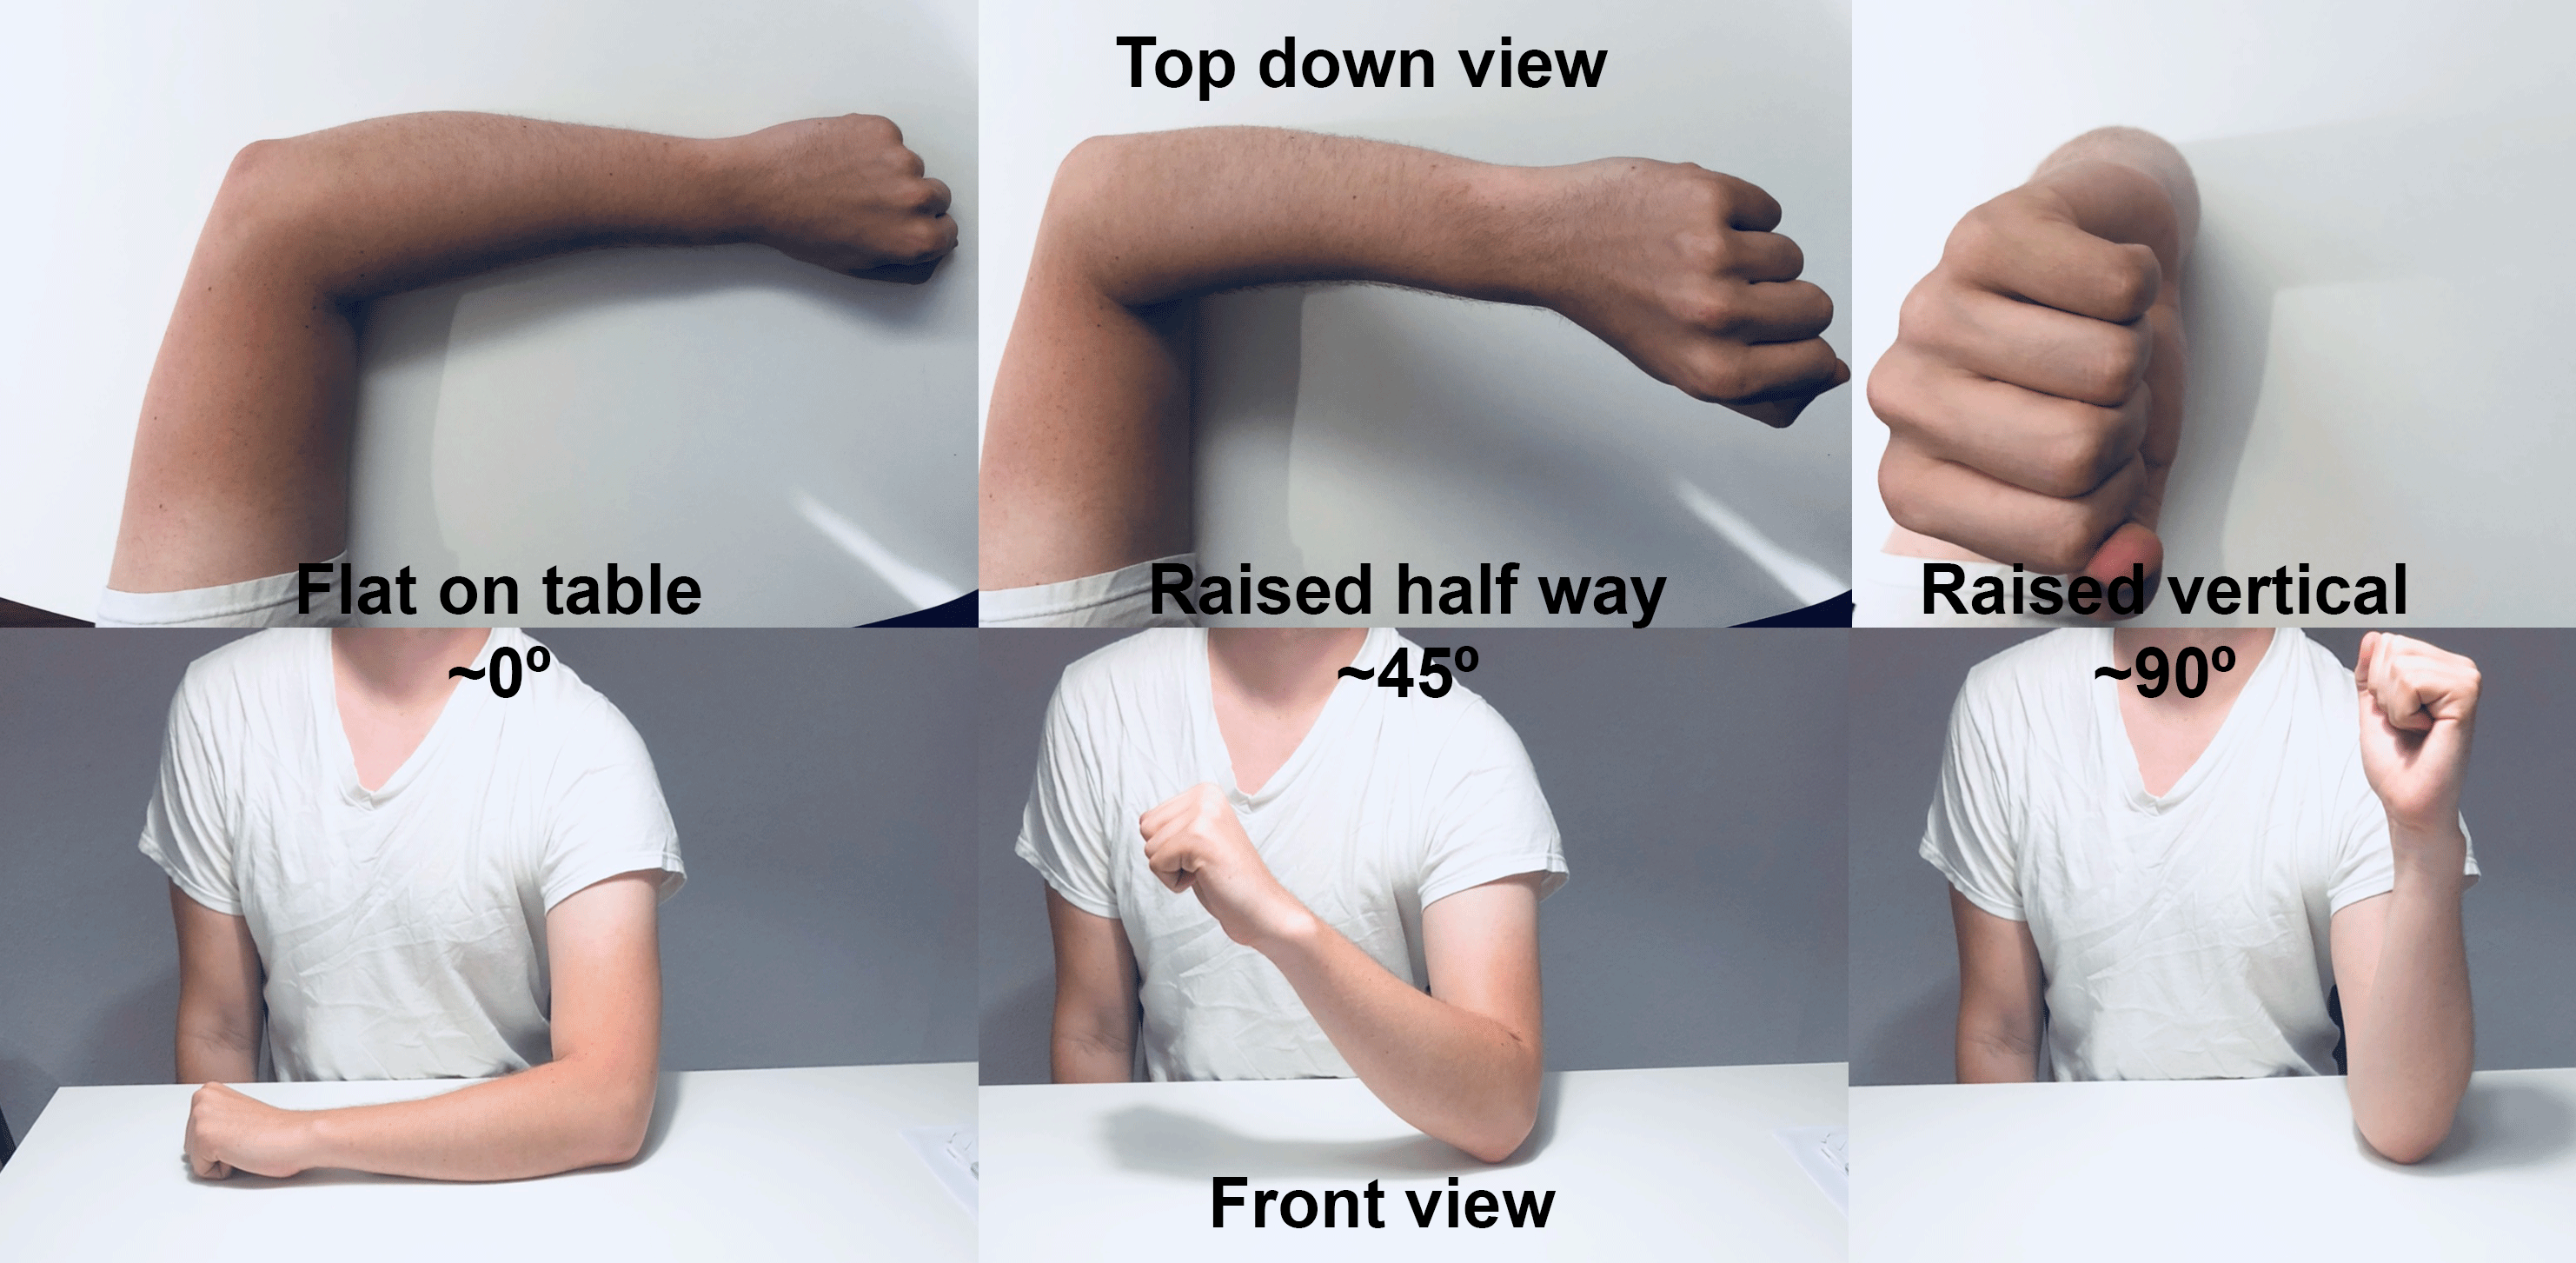
\includegraphics[width=1\textwidth]{figures/pitch.png}
    \caption{The movement for adjusting \underline{pitch} by rotating the arm around the elbow}
    \label{pitch}
\end{figure}

Roll is changed by rotating the wrist/lower arm, the angle between the back of the hand and table is then the measurement for this rotation.

\begin{figure}[h!]
    \centering
    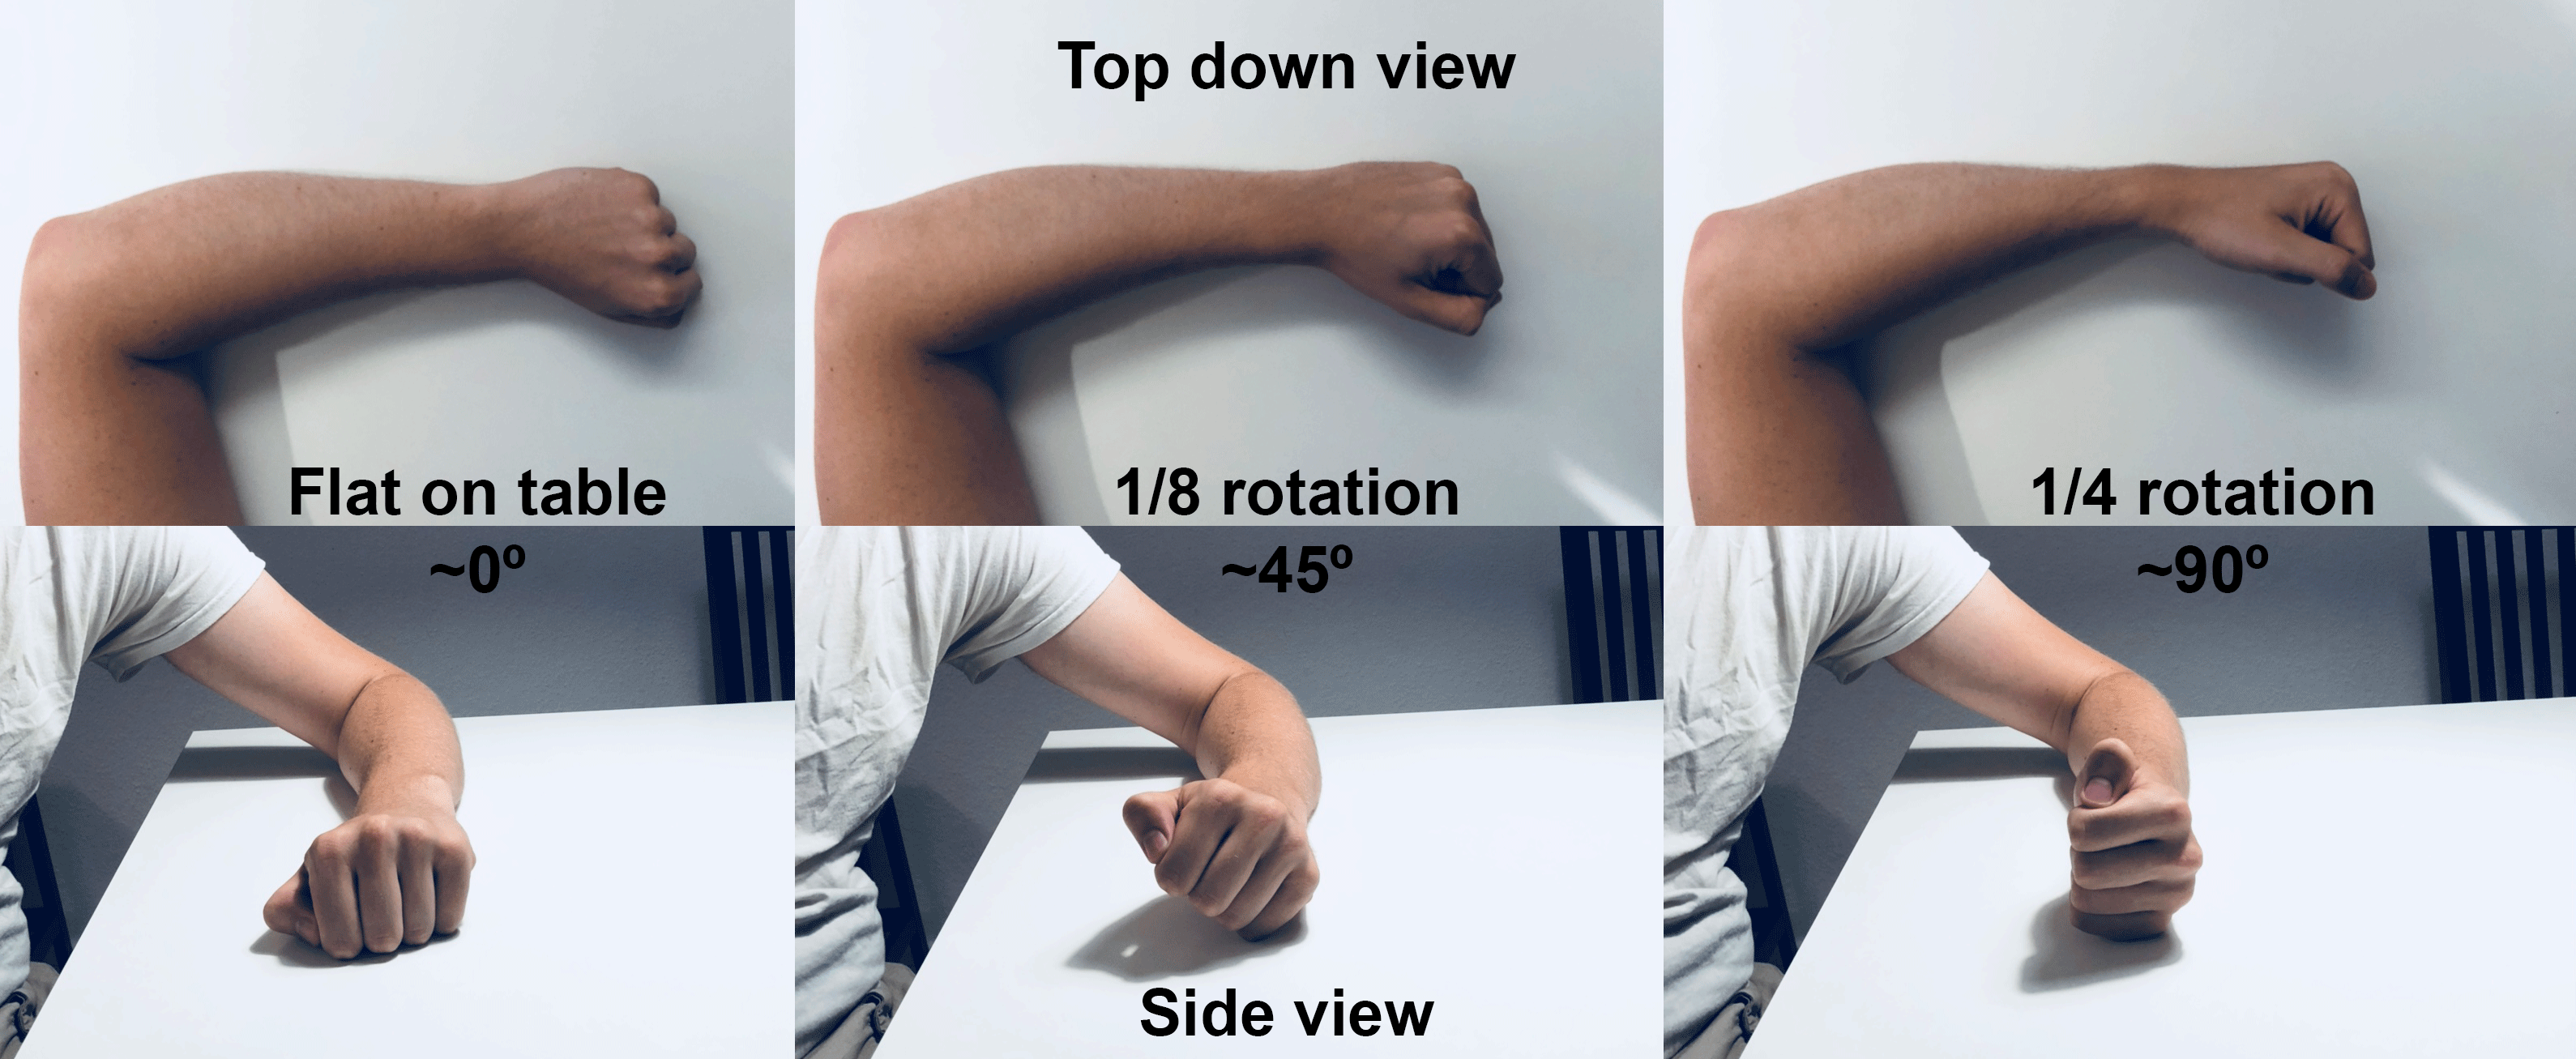
\includegraphics[width=1\textwidth]{figures/roll.png}
    \caption{The movement for adjusting \underline{roll} by rotating the wrist/lower arm}
    \label{roll}
\end{figure}

Yaw is changed by bending the lower arm the elbow, keeping it level with the table, thus changing the direction of the lower arm. The angle of direction is then the measurement for this rotation.

\begin{figure}[h!]
    \centering
    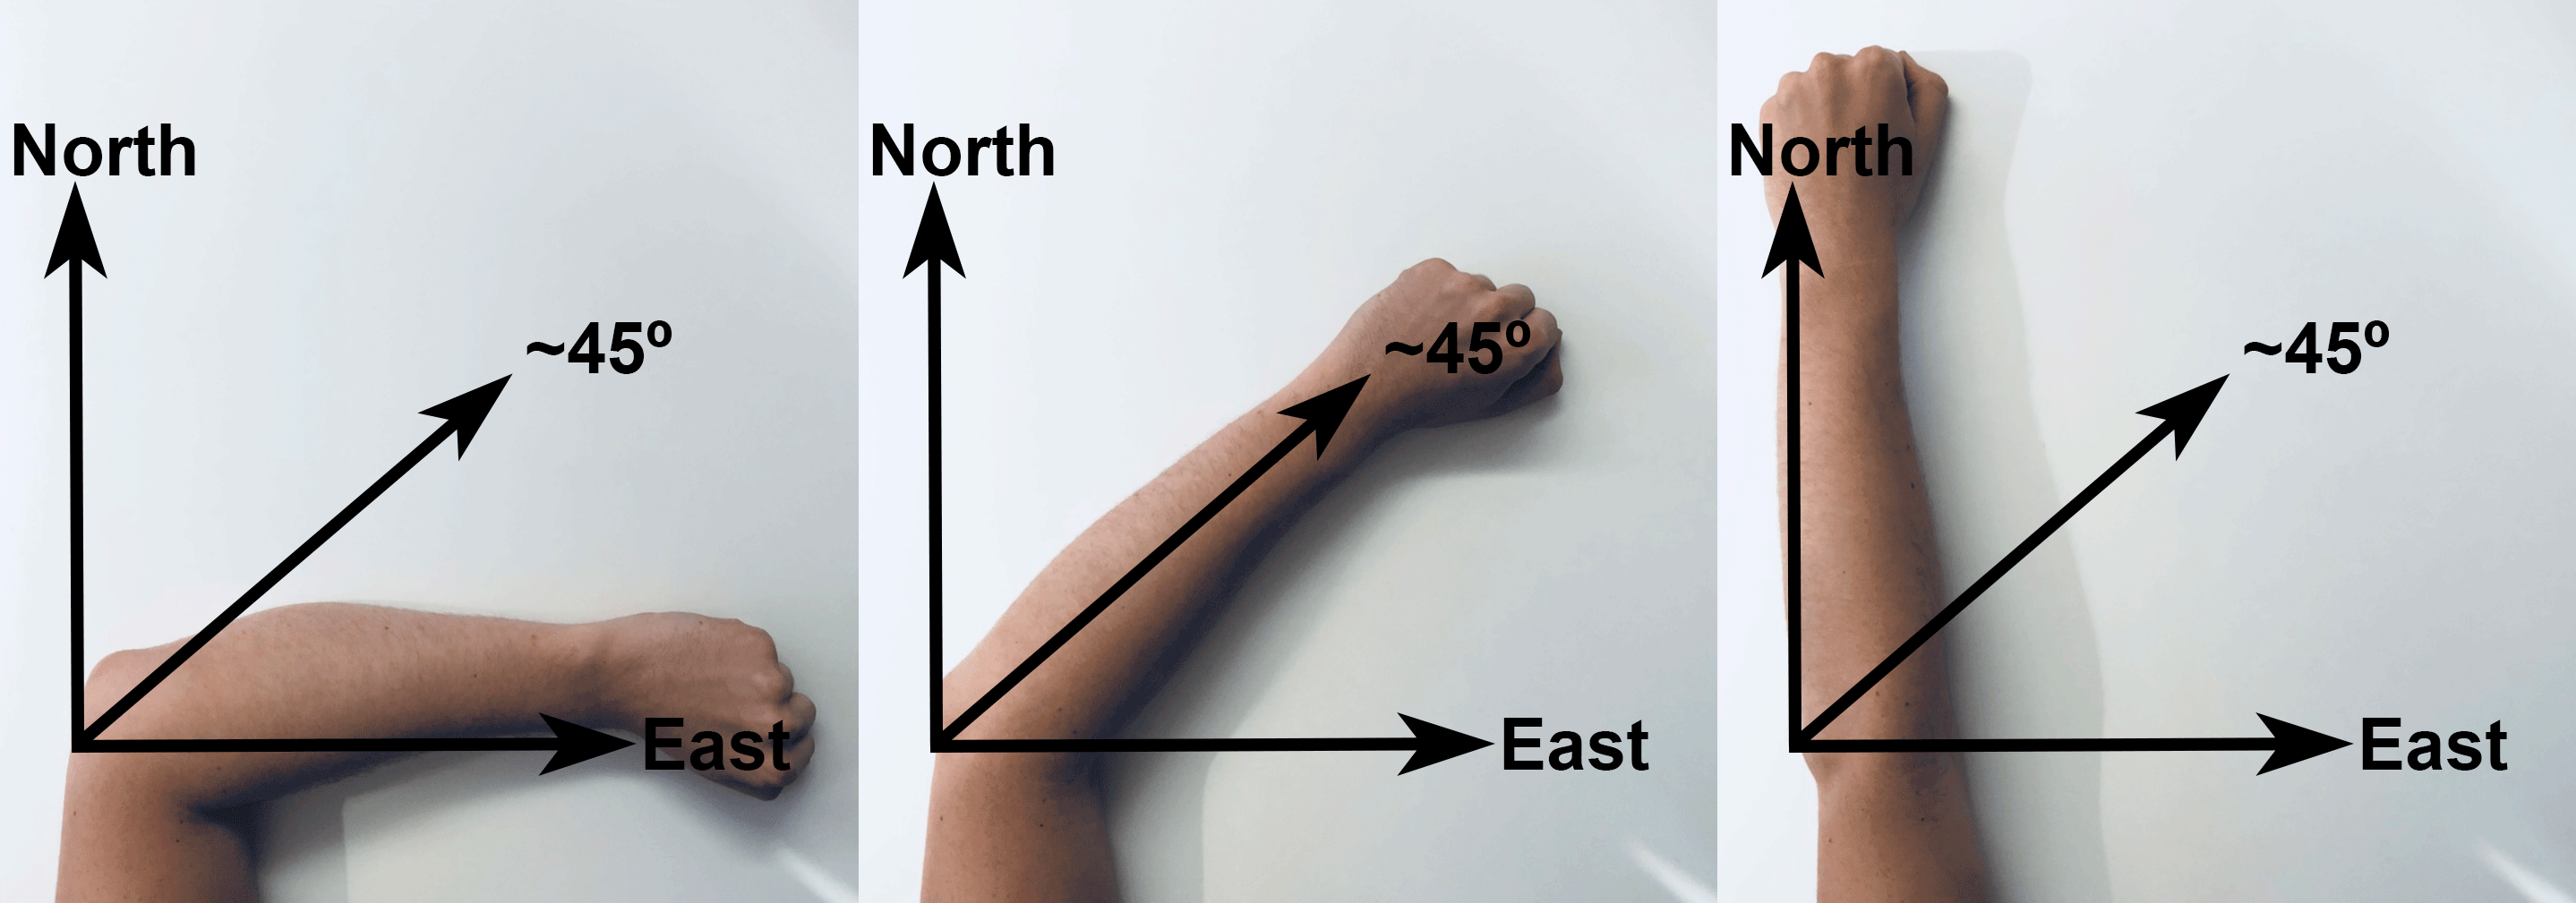
\includegraphics[width=1\textwidth]{figures/yaw.png}
    \caption{The movement for adjusting \underline{yaw} by rotating the lower arm around the elbow (note the arm is flat/horizontal on the table)}
    \label{yaw}
\end{figure}

Of course all three rotation can be achieved in other ways, for example yaw can be changed by turning the entire body to face another directions. But for the purpose of this thesis we look at these motions because they are done in front of one self, can be executed both while sitting at a table (for best reference) or while standing, and for all these motions the body itself also is a reference point, where turning your entire body would require another reference point to make sense of the scale.

\subsection{IMU}
\textbf{COMMENT: Get a illustration of the BNO055 or specs. Mention processing of data required - calibration issues.. Drift experiment}

In order to measure the orientation we will mount a device on the wrist which contains an IMU from which the orientation can be read. Most IMUs are equipped with accelerometers, gyroscopes and magnetometers and offers either raw sensor values or the calculated Euler angles and quaternions for absolute orientation. In it self the raw sensor values can't provide the orientation, since it measures the change for example will the gyroscope alone measure the rate of rotation witch in it self can't lead to an absolute orientation. But together the sensors provide enough data that this can be calculated. The IMU will use its magnetometer to find north and use this to calibrate yaw, using its accelerometers the IMU can measure gravity and calibrate both pitch and roll. All together this lets the IMU calculate the absolute orientation. These calculations also requires the IMU to be calibrated and if not done correctly this can lead to issues, such as drift, where the orientation values will change even though the IMU sits completely still. 

To demonstrate this, a test was preformed with the Adafruit 9-DOF Absolute Orientation IMU Fusion Breakout - BNO055\cite{gyro}, logging the Euler angles with and without calibration while the IMU sat completely still. Once every minute the Euler angles was read from the IMU and logged to a file, two trials where run for nine and twelve hours respectively without and with calibration. The results can be seen in Figure \ref{drift1} and \ref{drift2}, we see that without calibration the sensor drifts and the Euler angles change quite dramatically over time, while with calibration the Euler angles only had minor change.

\begin{figure}[h!]
    \centering
    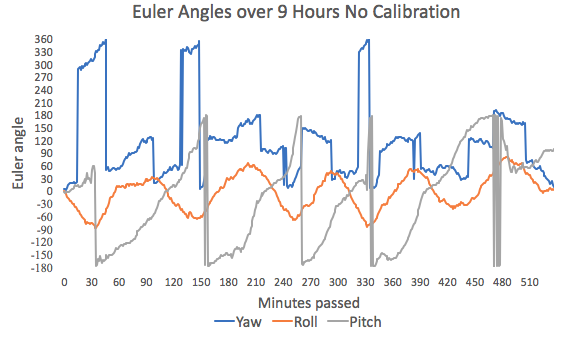
\includegraphics[width=1\textwidth]{figures/drift1.png}
    \caption{Reading the Euler angles from the BNO055 IMU\ref{gyro} without calibration}
    \label{drift1}
\end{figure}

\begin{figure}[h!]
    \centering
    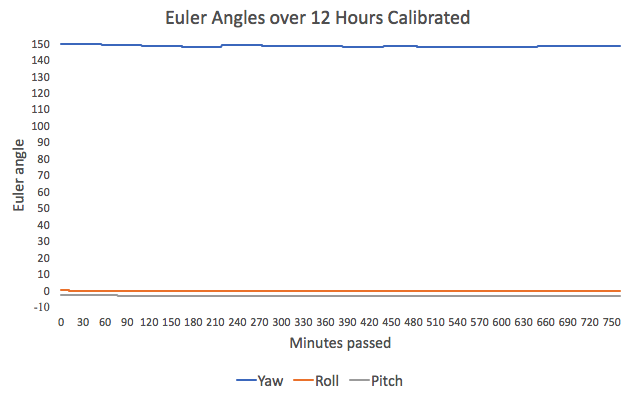
\includegraphics[width=1\textwidth]{figures/drift2.png}
    \caption{Reading the Euler angles from the BNO055 IMU\ref{gyro} with calibration}
    \label{drift2}
\end{figure}


The most common ways to represent absolute orientation is using either Euler angles\cite{euler} or quaternions\cite{quat}. Euler angles describes the orientation by angles of the 3 axis, this is the most intuitive approach but it has it downfall. When two of the gimbals in a gyroscope align into a parallel configuration, then one of the three degrees of freedom is lost, this is called Gimbal lock\cite{gimbal}. When Gimbal lock occurs changes in the locked axis cannot be measured, in order to fix it the axis which aligned itself with the other must be changed to get out of alignment and thus getting back the lost degree of freedom. This problem is often experienced in animation, where by defining movement only by total change in the three axis can cause strange and unintended results. The solution is to use quaternions, which is a mathematical number system which can represent the orientation of an object. Not getting into the math behind quaternions, but they solve the gimbal problem and quaternions can be transformed into Euler angles. Luckily when measuring the angles for the arm movements described gimbal lock does not occur, since the different axis does not come close to alignment in any position within the described movement. 


\subsection{Problems with yaw}
As described when measuring absolute orientation, then the magnetic north is used as the calibration point, meaning that 0º yaw will be pointing north, 90º pointing east and so on. Both pitch and roll is relative to the ground (horizontal plane), therefor no matter the yaw orientation you can get an absolute reading based on one point within the arm movement described earlier, e.g. you can rotate your wrist to a desired angle and take one measurement and know the orientation in that axis. This can't be done for yaw, it would require that you either first align yourself to a specific direction (north for example), and then bend the lower arm out in front to the desired angle, or it requires two measurement (one in the starting position, and one in the desired position) in order to calculate the difference, and achieve the desired angle. For this reason using the yaw orientation will not be investigated further, since it would introduce a higher burden for the user.